\documentclass[UTF8]{article}
\usepackage{ctex}
\usepackage{amsmath}
\usepackage{graphicx}
\usepackage{listings}
\usepackage{xcolor}
\usepackage{geometry}
\usepackage{textcomp}
\usepackage{subfigure}
\geometry{left=3.8cm,right=3.8cm}
\definecolor{dkgreen}{rgb}{0,0.6,0}
\definecolor{gray}{rgb}{0.5,0.5,0.5}
\definecolor{mauve}{rgb}{0.58,0,0.82}

\lstset{ %
	language=java,                % the language of the code
	basicstyle=\footnotesize,   % 代码字体大小
	numbers=left,                   % where to put the line-numbers
	numberstyle=\tiny\color{gray},  % 行号颜色
	stepnumber=1,                   % 行行号隔几行标注一次
	numbersep=5pt,                  % how far the line-numbers are from the code
	backgroundcolor=\color{white},      % choose the background color. You must add \usepackage{color}
	showspaces=false,               % show spaces adding particular underscores
	showstringspaces=false,         % underline spaces within strings
	showtabs=false,                 % show tabs within strings adding particular underscores
	frame=single,                   % adds a frame around the code
	rulecolor=\color{black},        % if not set, the frame-color may be changed on line-breaks within not-black text (e.g. commens (green here))
	tabsize=2,                      % 行首和边框的距离
	captionpos=b,                   % sets the caption-position to bottom
	breaklines=true,                % sets automatic line breaking
	breakatwhitespace=false,        % sets if automatic breaks should only happen at whitespace
	title=\lstname,                   % show the filename of files included with \lstinputlisting;
	% also try caption instead of title
	keywordstyle=\color{blue},          % keyword style
	commentstyle=\color{dkgreen},       % comment style
	stringstyle=\color{mauve},         % string literal style
	escapeinside={\%*}{*)},            % if you want to add LaTeX within your code
	morekeywords={*,...}              % if you want to add more keywords to the set	
}

\begin{document}
	\title{黑白棋游戏}
	\author{陈璐 181250012 chenlu@smail.nju.edu.cn}
	
	\maketitle
	
	\tableofcontents
	
\section{MiniMax搜索实现}
\subsection{基本思想}
	\indent MiniMax算法的主要思想为:假定对手会选择所有可选择行动中最有利于对方的选择,在此基础上,选择对自己最有利的行为,具体而言,在每个状态中,agent都选择最坏情况下能够带来最优收益的行动,而每个行动的收益为执行此行动后所进入的次态的value,每个状态的value通过下式计算:\\
	\begin{footnotesize}
		\begin{equation}
		MiniMax(s)=
		\begin{cases}
		UTILITY(s) & if\ TERMINAL-TEST(S) \\ 
		max_{a\in ACTION(s)}MINIMAX(RESULT(s,a))& if\ PLAYER(s)=MAX \\ 
		min_{a\in ACTION(s)}MINIMAX(RESULT(s,a))& if\ PLAYER(s)=MIN \\
		\end{cases}
		\end{equation}
	\end{footnotesize}

	\indent 由于此游戏规模较大,搜索到最终状态所需的时间过长,因此,可对(1)式进行修改,使其在游戏结束时或搜索到一定深度后就通过一启发式函数返回对状态的估计值。\\
	\indent 综上所述,基于上述式子和贪心的思想,即可编写程序对应实现。

\subsection{主要实现过程}
	\indent 对于此程序,可以将其内容与上一小节所描述的过程进行一一对应,主要分为计算value值和贪心选取最优行动两个部分。
	
	\indent\textbf{1、计算状态对应的value}
	\begin{lstlisting}[caption=计算每个状态对应的value]
	public float miniMaxRecursor(State state, int depth, boolean maximize) {
			if (computedStates.containsKey(state)) 
					return computedStates.get(state);
			if (state.getStatus() != Status.Ongoing)
					return finalize(state, state.heuristic());
			if (depth == this.depth)
					return state.heuristic();
			float value = maximize ? Float.NEGATIVE_INFINITY : Float.POSITIVE_INFINITY;
			int flag = maximize ? 1 : -1;
			List<Action> test = state.getActions();
			for (Action action : test) {
					try {
							State childState = action.applyTo(state);
							float newValue = this.miniMaxRecursor(childState, depth + 1, !maximize);
							if (flag * newValue > flag * value) 
						  			value = newValue;
					} catch (InvalidActionException e) {
							throw new RuntimeException("Invalid action!");
					}
			}
			return finalize(state, value);
	}
	\end{lstlisting}
	\indent 此函数用于计算每个状态的value值,主要实现了对(1)式中3种不同情况进行讨论:\\
	\indent 1、结束搜索(line 4-7):当游戏结束或者到达设置深度时,即返回此状态对应的value。\\
	\indent 2、递归计算子状态,以对当前状态进行评估(line 8-21):判断当前执行行动的为max还是min(line 8-9),并计算次态的value(line 14),最后选择可以选择的最优value值作为当前结点的value,返回此值。\\
	\indent\textbf{2、贪心选择最优行动}
	\begin{lstlisting}[caption=贪心选取最优行动]
	public Action decide(State state) {
			float value = maximize ? Float.NEGATIVE_INFINITY : Float.POSITIVE_INFINITY;
			List<Action> bestActions = new ArrayList<Action>();
			int flag = maximize ? 1 : -1;
			for (Action action : state.getActions()) {
			try {
					State newState = action.applyTo(state);
					float newValue = this.miniMaxRecursor(newState, 1, !this.maximize);
					if (flag * newValue > flag * value) {
						value = newValue;
						bestActions.clear();
					}
					if (flag * newValue >= flag * value) bestActions.add(action);
			} catch (InvalidActionException e) {
					throw new RuntimeException("Invalid action!");
					}
			}
			// If there are more than one best actions, pick one of the best randomly
			Collections.shuffle(bestActions);
			return bestActions.get(0);
	}
	\end{lstlisting}
	
\indent 此过程和计算value时的过程类似,不同的是,在获得所有次态的value后,miniMaxRecursor过程对当前状态value进行更新,而decide过程只选择最优次态所对应的行动,并返回此行动。
	
\subsection{实现细节}
\indent\textbf{1、使用置换表,避免对状态进行重复计算}\\
\indent 算法将已经计算过的状态和所对应的value值保存起来,在每次计算状态的value时,首先判断此状态是否已被计算(listing1 line2-3),如果已经被计算,则直接返回此状态的value,如果未被计算,则在计算结束后将此状态和对应value储存起来(line 21),以供后续使用,从而避免了多次对同一状态进行计算,以一定的空间代价换取搜索时间的缩减。\\
\indent 在此处,已被计算的状态和其对应的value主要通过map数据结构进行存储,经过查询得知,JAVA中map的实现原理为hash,而其被理论上证明,在基于一定假设的情况下,插入元素和查找元素两个操作的均只需要常数时间代价,因此整体而言效率较高。\\
\indent 但令人困惑的是,作者注释掉了存储操作,并标注上"THIS IS BROKEN DO NOT USE" 来告诉使用者不要使用此功能,不过经过测试,去掉注释后程序依旧运行正常,因此,不明白作者的用意何在。\\
\indent 如果我们假设插入和查找功能被正确实现,设置最大深度为5,进行测试,不使用此功能时,单次决策时间平均约为146.7ms,使用此功能时,为17.8ms,因此置换表能够有效地减少搜索时间。\\
\indent 在后续的所有实现过程中,我们仍按照作者的意思将其注释掉,不去使用它,分析时也不考虑它所带来的影响。\\
\begin{lstlisting}[caption=存储state-value pair]
private float finalize(State state, float value) {
		// THIS IS BROKEN DO NOT USE
		//computedStates.put(state, value);
		return value;
}
\end{lstlisting}

\indent\textbf{2、通过一个简单的指示位避免了对max和min状态的判断}\\
\indent 按照(1)式的过程,在为min回合时,选择最小值,在max回合时,选择最大值,而实际上,所有元素的最小值对应的为所有元素取负后的最大值,因此设置标志位flag(line 4),在max回合时其为1,比较时不取负,按照原值比较,选取其中最大值,在min回合时其为-1,比较时取负(乘以flag),按照取负后的值比较,选取最大值,也就是原最小值。

\section{AlphaBeta剪枝}
\subsection{实现过程}
\indent 修改miniMaxRecursor过程,在参数列标中加入preval,用于表示当前父节点的最优值,也即是过程内原本就存在的value变量中的值,在每次循环过程中进行判断,由于当前循环中value中的值在不断向不利于父节点的方向发展(如父节点为max,子结点的value就不断减小,父节点为min,子节点的value就不断增大),因此,只要子节点目前的值劣于父节点已经可以获得的最优值,那么就无需对此子节点的后续结点进行搜索,而是直接进行剪枝,返回当前获得的值,由于此值劣于最优解,因此对最终结果不造成影响,具体实现过程如下所示。
\begin{lstlisting}[caption=alphabeta剪枝]
for (Action action : test) {
		try {
				State childState = action.applyTo(state);
				float newValue = this.miniMaxRecursor(childState, depth + 1, !maximize,value);
				if (flag * newValue > flag * value) 
						value = newValue;
		} catch (InvalidActionException e) {
				throw new RuntimeException("Invalid action!");
		}
		if((0-flag) * value <= (0-flag) * preval) return value; //2
}
\end{lstlisting}

\indent 如上所示,剪枝过程在listing4的第10行,其中0-flag表示其父节点的flag值,此判断语句的意思是:由于value值在不断向不利于父节点的方向变化,因此,如果当前值不优于父节点值,那么在整个循环中,value的值都不会优于父节点的值,即其不会对父节点进行更新,属于无用结点,因此停止探索,直接返回。

\subsection{性能分析}
\indent 不断增加最大深度,并统计单次决策时间,画出柱状图如图1所示,而当深度增加到7时,不进行剪枝时单次决策时间高达23s,已经严重影响了游戏的体验,因此此处只统计到深度为6的情形。\\
\indent 由此可见,在深度较小时,alphabeta剪枝已经能够取得较好的结果,能够将时间缩短至原来的一半,在深度较大时此剪枝方法优势更加明显,所需的决策时间不到原来的十分之一。

\begin{figure}[ht]
	\centering
	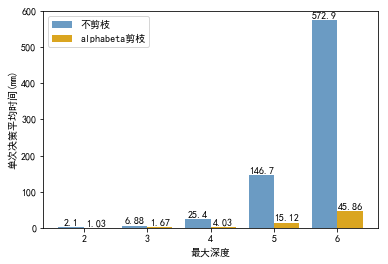
\includegraphics[width=8cm]{ab.png}
	\caption{alphabeta剪枝性能分析}
\end{figure}

\section{heuristic函数}
\subsection{函数分析}
\indent 阅读代码可发现,对于状态value值的预测为5部分的线性组合:\\
\indent 1、winconstant: 游戏获胜时的获得的奖励。\\
\indent 2、cornerDifferential: max一方占据的四个角落格子的数目于min方占据数目的差值。\\
\indent 3、moveDifferential: max可进行的行动数与min可进行的行动数目的差值。\\
\indent 4、pieceDifferential: max拥有棋子数与min拥有棋子数的差值。\\
\indent 5、stabilityDifferential: 能够翻转的棋子数目的差值。\\
\indent 以上五个参数被赋予不同的权值,表示对于其的重视程度,由于获胜优先级最高,因此其赋予了足够高的权重,为5000,同时,四个角落中棋子永远不可能被翻转,且角落元素对翻转两边界棋子以及对应对角线上棋子具有重要作用,因此优先级也较高,赋予权值为300,其余三种作为不算非常重要的考量因素,分别赋予权值8,1,1。

\subsection{改进}
\indent 研究黑白棋的游戏规则,以及参考游戏策略后,可以提出以下改进:\\
\indent 1、由于边缘位置往往比中间位置更好,因此可以加入edgeDifferential,用来衡量边缘棋子数目的差值,赋予权重20。\\
\indent 2、在游戏中发现,如果对角线上最靠近角落(不为角落)位置被我方填入,那么对方则可以较为轻易填入对角线位置,因此加入diacornerDifferential,用以计算此位置棋子数目的差值,赋予权重80。\\
\indent 3、在游戏进行到后期,也即决定胜负的关键时期,注意到有些棋子已经不可能被翻转了,因此这些棋子必定作为最终我们的得分的一部分,因此加入fixDifferential,用来计算不能翻转的棋子的数目的差值,赋予权重60.\\
\indent 因此,修改后的heuristic函数如listing5所示。

\begin{lstlisting}[caption=改进后的heuristic函数]
public float heuristic() {
		Status s = this.getStatus();
		int winconstant = 0;
		switch (s) {
				case PlayerOneWon:
						winconstant = 5000;
						break;
				case PlayerTwoWon:
						winconstant = -5000;
						break;
				default:
						winconstant = 0;
						break;
		}
		return this.pieceDifferential() +
		8 * this.moveDifferential() +
		300 * this.cornerDifferential() +
		1 * this.stabilityDifferential() + 
		20 * this.edgeDifferential() +
		80 * diacornerDifferential() +
		60 * fixDifferential() +
		winconstant;
}
\end{lstlisting}

\section{MTDDecider类}
\subsection{实现过程}
\indent 本算法主要采用零宽窗口策略,使用二分法不断确定结点的估值,从而使得尽可能最大化地进行剪枝。\\
\indent\textbf{1、零宽窗口策略}:在进行alpha-beta剪枝时,由于alpha值单调不减,beta值单调不增,因此,只有alpha<value<beta地结点才是有效结点,其余结点均为无效结点。基于此思想,我们使得窗口,即beta-alpha的值尽可能小,从而能够尽可能最大化地实现剪枝。因此我们设置窗口为alpha,alpha+1(或bete-1,beta,这取决于当前结点为max结点还是min结点),即为零宽窗口,如果返回值小于alpha,说明此结点为无用结点,进行剪枝,如果大于等于alpha+1,则用此value值更新alpha,并重复上述过程,直到无法更新为止。由于搜索宽度极小,因此单次搜索时间大大缩短。\\
\indent\textbf{2、MTDF算法}:MTD采用了上述零宽窗口的策略,在计算每个结点的value值时,维护一个value的上下界,并分别初始化为正无穷和负无穷,每次围绕范围内的一个猜测g来进行零宽搜索(AlphaBetaWithMemory过程),如果返回值大于猜测值g,则由于下界单调不减,因此降下界更新为g,如果返回值小于猜测g,则将上界更新为g,从而使得value的可能返回变小,直至收敛于一个准确值,此值即为真实的value值,并进行返回。\\
\indent\textbf{3、置换表}:由于我们可能会对一个结点进行多次搜索,因此采用置换表方法,将已经计算过的结点信息储存起来,之后再访问此结点时只需要从内存种取出此信息,而无需重复计算,置换表的本质是哈希表,在理论上能够实现O(1)的存数据和取数据操作,因此能够大大提高搜索速度。

\subsection{与MiniMaxDecider类的异同分析}
\indent\textbf{相同点}:MTDF基于MiniMax算法,都是采用深度优先搜索的基本思想,并对搜索深度进行限制,在到达一定深度后采用启发式函数对当前状态进行估计。\\
\indent\textbf{不同点}:MTDF算法对MiniMax进行了改进,引入了alpha-beta剪枝,并且采用二分思想使剪枝更快进行,同时还应用了置换表以避免重复搜索,算法效率相较于MiniMax算法有了较大提升。\\

\end{document}




